%%%%%%%%%%%%%%%%%%%%%%%%%%%%%%%%%%%%%%%%%%%%%%%%%%%%%%%%%%%%%%%%%
%%% %
%%% % weiiszablon.tex
%%% % The Faculty of Electrical and Computer Engineering
%%% % Rzeszow University Of Technology diploma thesis Template
%%% % Szablon pracy dyplomowej Wydziału Elektrotechniki 
%%% % i Informatyki PRz
%%% % June, 2015
%%%%%%%%%%%%%%%%%%%%%%%%%%%%%%%%%%%%%%%%%%%%%%%%%%%%%%%%%%%%%%%%%

\documentclass[12pt,twoside]{article}

\usepackage{raport}

\author{Damian Bielecki}
\definechangesauthor[name=Paweł P., color=blue]{PP}
% np. EF-123456, EN-654321, ...
\studentID{ME-163461}
\title{Implementacja sterowania hierarchicznego mobilnym robotem kołowym z wykorzystaniem języka Python}
\titleEN{Temat pracy po angielsku}


%%% wybierz rodzaj pracy wpisując jeden z poniższych numerów: ...
% 1 = inżynierska	%BSc
% 2 = magisterska	%MSc
% 3 = doktorska		%PhD
%%% na miejsce zera w linijce poniżej
\newcommand{\rodzajPracyNo}{1}


%%% promotor
\supervisor{dr \added[id=PP]{inż.} Paweł Penar}

%%% promotor ze stopniami naukowymi po angielsku
\supervisorEN{(academic degree) Imię i nazwisko opiekuna}

\abstract{Treść streszczenia po polsku}
\abstractEN{Treść streszczenia po angielsku}

\begin{document}

% strona tytułowa
\maketitle

\blankpage

% spis treści
\tableofcontents
\clearpage
\blankpage

\section{Wprowadzenie}
Od lat można zauważyć zwiększająca się popularność różnych robotów, które bazując na wprowadzonej do systemu mapie
autonomicznie poruszają się po terenie tak aby osiągnąć określony cel.
Celem projektu inżynierskiego będzie zaimplementowanie algorytmu wyszukującym najkrótszą ścieżkę.
Do przetestowania algorytmu zostanie napisany prosty program symulujący robota poruszającego się po wyznaczonej ścieżce.
Kolejnym etap projektu to zbudowanie robota mającego zweryfikować zaproponowaną przez algorytm ścieżkę. 

Głównym powodem podjęcia się implementacji takiego algorytmu jest chęć zapoznania się z systemami planującymi ruch robota
i próba zaimplementowania takiego rozwiązania na fizycznym robocie.

% Potencjalne zastosowania autonomicznych są 
\replaced[id=PP]{
	Ze względu na cel projektu inżynierskiego oraz powód jego realizacji, przyjęto, że praca będzie złożona z przeglądu literatury, implementacji i symulacji algorytmu A* w języku Python oraz weryfikacji przyjętych rozwiązań obiekcie rzeczywistym.
}{\textbf{Na zakres pracy składa się: ..... }
%\begin{itemize}
%	\item Przegląd literatury
%	\item Implementacja algorytmu A* w języku Python
%	\item Symulacja działania pracy algorytmu
%	\item Weryfikacja na obiekcie rzeczywistym
%\end{itemize}
}

\replaced{Mając na uwadze zakres pracy, jej treść podzielono na szereg rozdziałów. 
Rozdział pierwszy stanowi przegląd literatury oraz istniejących rozwiązań, które będą podstawą założeń przyjętych we opracowywanym rozwiązaniu. Rozdział drugi skupia się na genezie, charakterystyce i opisie działania wybranego algorytmu wyszukiwania najkrótszej ścieżki. Dodatkowo zostaną przedstawione inne algorytmy zwiększającą autonomie robota mobilnego. Rozdział trzeci przedstawia własną implementacje algorytmu A* oraz środowisko symulacyjne w języku Python. Kolejny rozdział to omówienie budowy robota mobilnego oraz jego programu sterującego. W tym kontekście szczególną uwagę poświęcono komunikacji oraz sterowaniu silnikami Rozdział piąty stanowi podsumowanie pracy i przedstawia przeprowadzone testy wykonane w środowisku symulacyjnym oraz rzeczywistym. }{
\textbf{Omówienie rozdziałów}

Rozdział pierwszy - zawiera przegląd literatury oraz istniejących rozwiązań. 
Na ich podstawie określona zostanie ogólna struktura własnego rozwiązania.

Rozdział drugi - skupia się na genezie, charakterystyce i opisie działania wybranego algorytmu wyszukiwania najkrótszej ścieżki.
Dodatkowo zostaną przedstawione inne algorytmy zwiększającą autonomie robota mobilnego.

Rozdział trzeci - w tym rozdziale zostanie przedstawiony napisany algorytm oraz środowisko symulacyjne w języku Python.

Rozdział czwarty - omawia budowę robota mobilnego oraz jego program sterujący.
W szczególności skupiono się na komunikacji oraz sterowaniu silnikami.

Rozdział piąty - przedstawia przeprowadzone testy wykonane w środowisku symulacyjnym oraz rzeczywistym. }

\section{Przegląd literatury}

\section{Algorytm A*}
\subsection{Geneza powstania}
Algorytm A* powstał w ramach projektu Shakey, zapoczątkowanego w 1966 roku przez Charles Rosen'a.
Celem projektu było zbudowanie robota, który potrafiłby planować własne działania. 
Zbudowany robot wyróżniał się na tle innych tym że integrował kilka różnych modeli sztucznej 
inteligencji pracującej jako jeden system.

Robot został zbudowany z:
\begin{itemize}
	\item kamery telewizyjnej i dalmierza optycznego - system wizyjny do obserwacji środowiska
	\item łącza radiowego - służącego do komunikacji z bazą, odbierania i wysyłania komend
	\item detektora uderzeń - pozwalający na zatrzymanie robota w przypadku kolizji
\end{itemize}

Komunikacja odbywała się poprzez wysyłane radiowo, tekstowe polecenia mające określoną strukturę np.:
GOTO D4 - co oznaczało automatyczne przemieszczenie się robota do wskazanej pozycji
\begin{figure}[H]
	\centering
	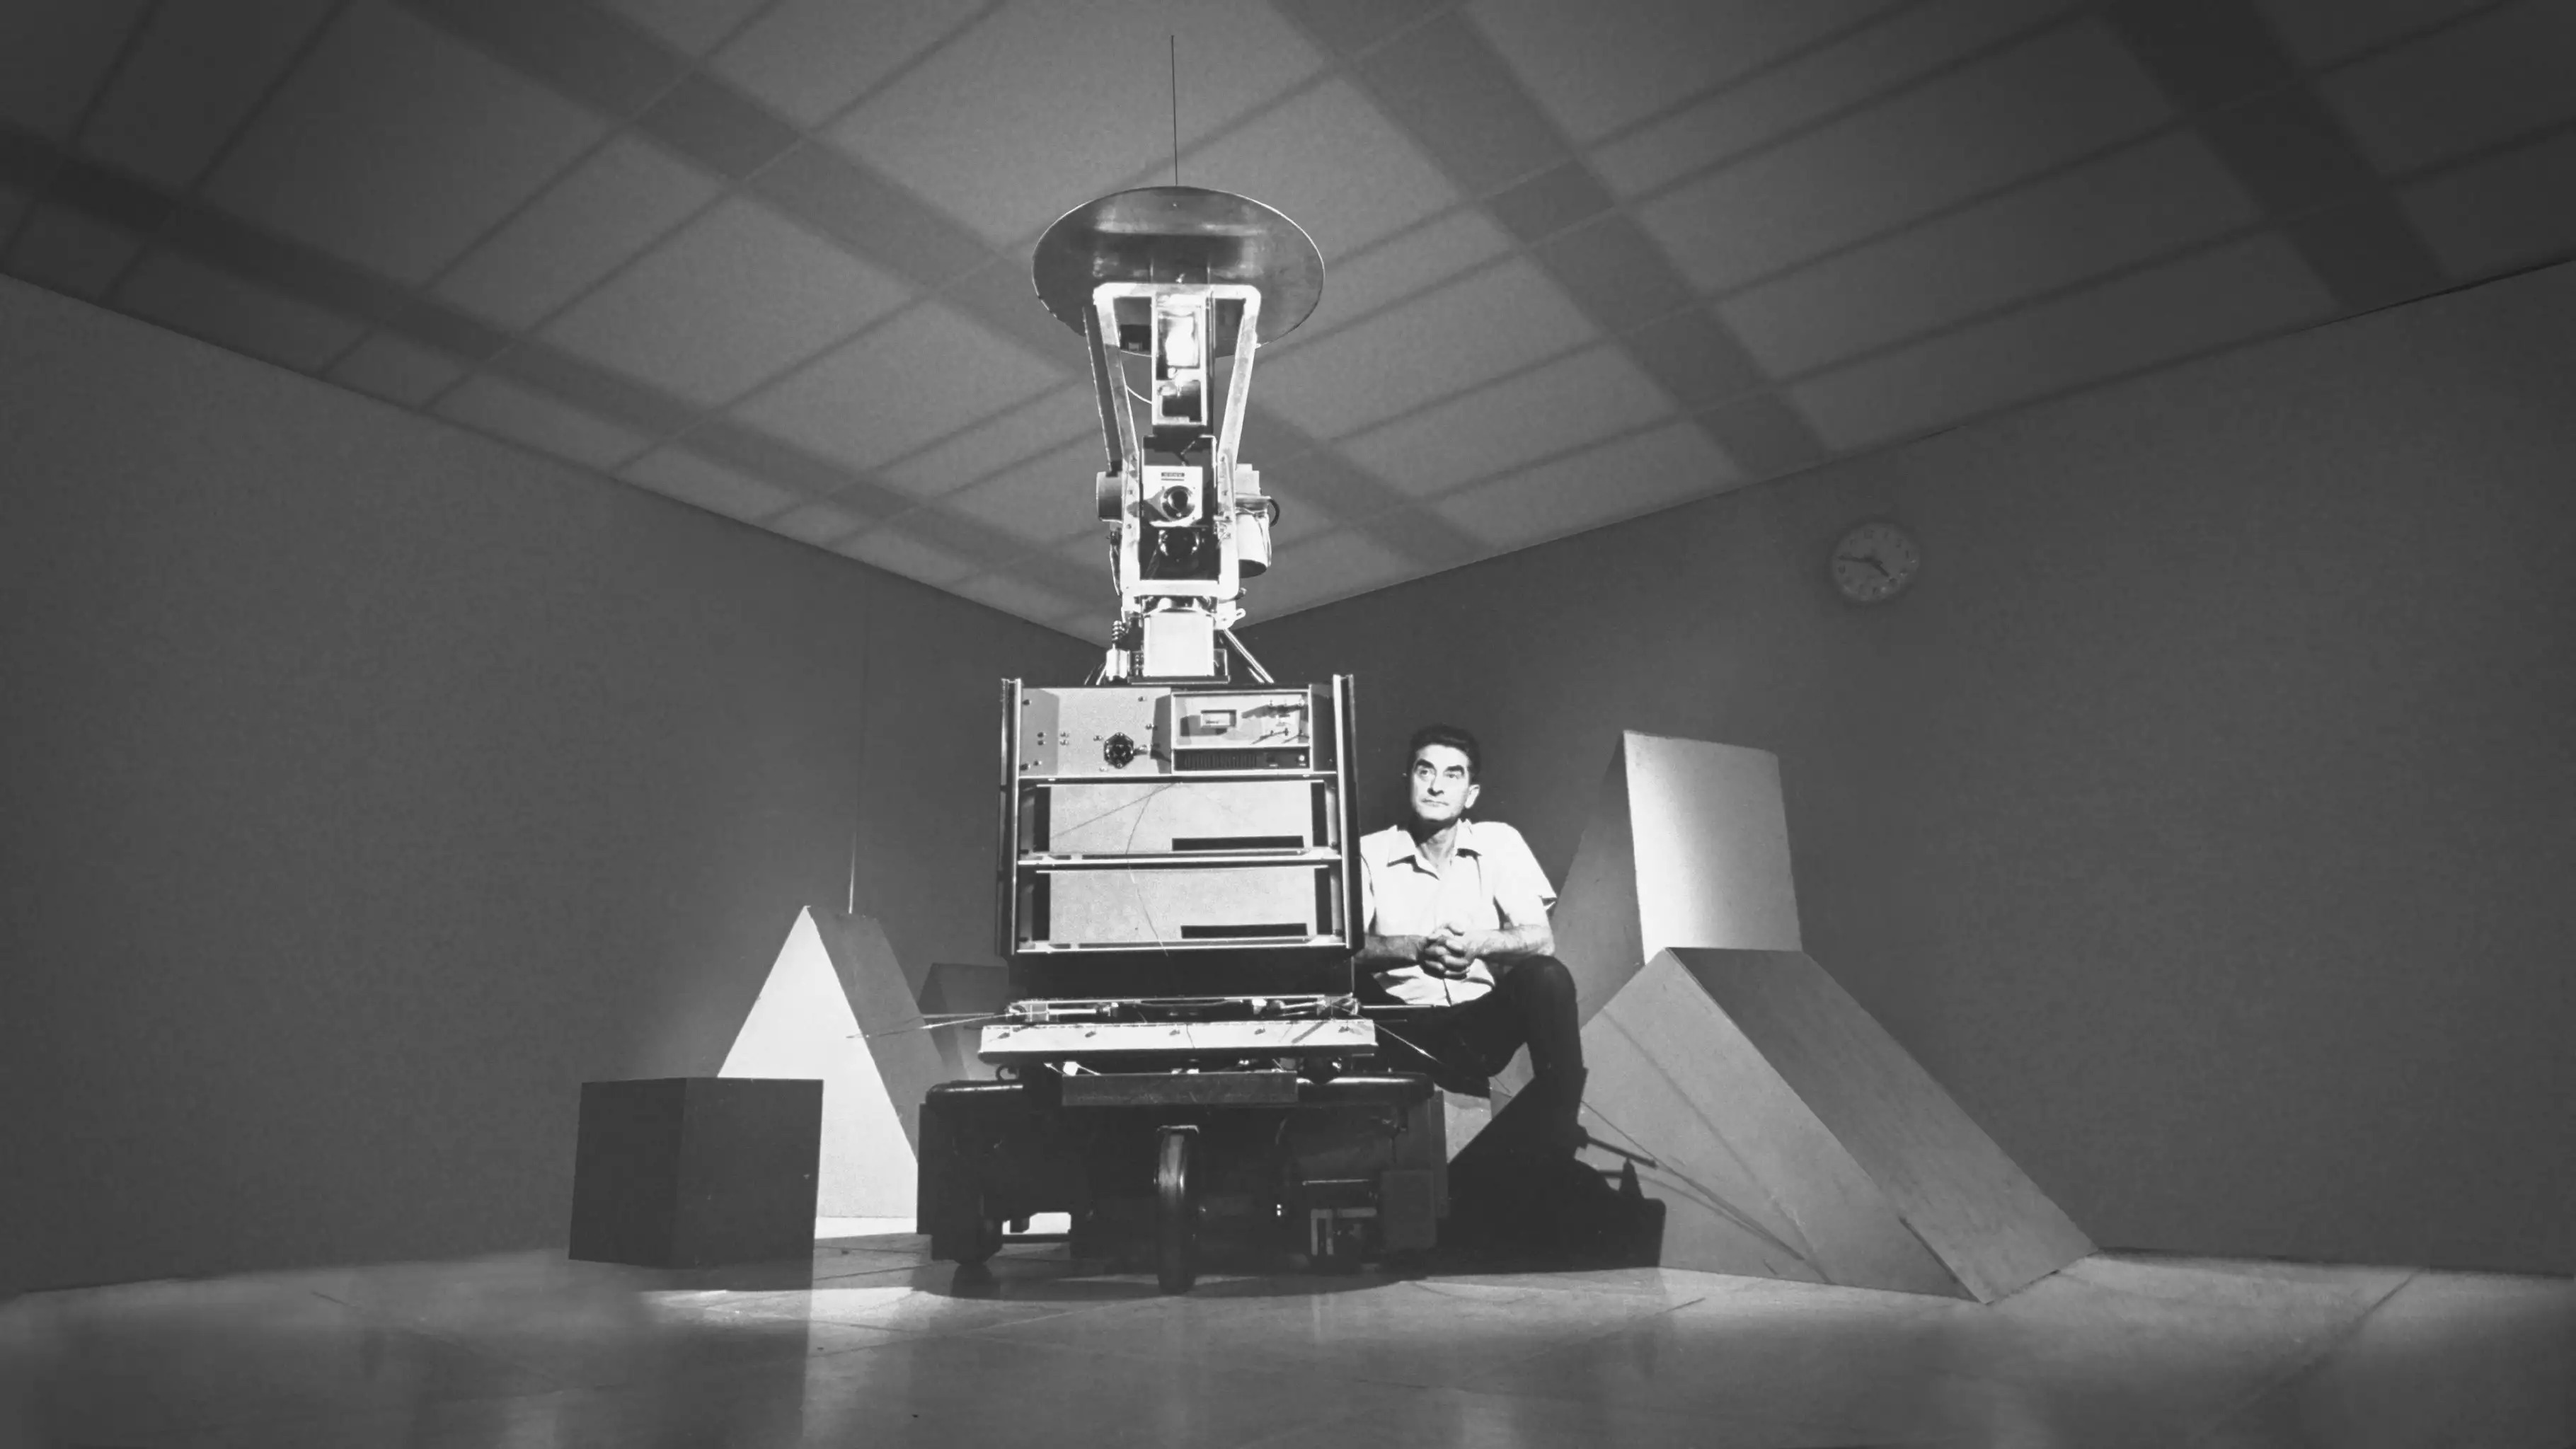
\includegraphics[width=14cm]{pages/algorytm/zdjecia/shakey2.jpg}
	\caption{Robot Shakey i Charles Rosen, inicjator projektu \cite{robotShakey}}
	\label{fig:Rys}
\end{figure}

\subsection{Opis działania algorytmu}

A* to heurestyczny algorytm wyznaczający najkrótszą możliwą ścieżkę w grafie. 
Jest to algorytm zupełny i optymalny, a więc zawsze zostanie wyznaczone optymalne 
rozwiązanie. Ze względu na przeszukiwanie oparte na grafie algorytm działa najlepiej na strukturze drzewiastej.
Zadaniem algorytmu jest minimalizacja funkcji:
\begin{equation}
	f(x)=h(x) + g(x)
	\label{Eq:funkcjaKosztuAStar}
\end{equation}
gdzie: $f(x)$ - minimalizowana funkcja, $g(x)$ - to rzeczywisty koszt dojścia do punktu x.

Funkcja $h(x)$ to funkcja heurestyczna, oszacowuje ona koszt dotarcia od punktu x do wierzchołka docelowego

Zalety:
\begin{itemize}
	\item jest kompletny i optymalny
	\item może przeszukiwać skomplikowane mapy
	\item jest najwydajniejszym takim algorytmem
\end{itemize}
Wady:
\begin{itemize}
	\item jego wydajność w znacznej mierze zależy od funkcji heurestycznej
	\item Każda akcja ma stały koszt wykonania
	\item nie nadaje się do często zmieniającego się otoczenia robota, wymaga ponownego przeliczenia
\end{itemize}


\textbf{Przykładowe funkcje heurestyczne:}
\begin{itemize}
	\item Funkcja euklidesowa
	      \begin{equation}
	      	h(x)= 10 * \sqrt[2]{(x_1 - x_2)^2 + (y_1 - y_2)^2}
	      	\label{Eq:heuresticEucalides}
	      \end{equation}
	\item Geometria Manhattanu (innaczej metryka miejska)
	      \begin{equation}
	      	h(x)= |x_2 - x_1| + |y_2 - y_1|
	      	\label{Eq:heuresticManhattanu}
	      \end{equation}
\end{itemize}
Gdzie: $x_1$ i $y_1$ to współrzędne wyznaczanego punktu, $x_2$ i $y_2$ to koordynaty celu


%TODO: cos o innych algorytmach np. skanowaine otoczenia lidarem



\section{Implementacja}

\subsection{Implementacja algorytmu}
Mechanizm wyszukiwania najkrótszej ścieżki został zamknięty w jednym module o nazwie aStar.
Na moduł składa się klasa AStar ze wszystkimi potrzebnymi metodami oraz klasa Node reprezentująca 
pojedynczy punkt przeszukiwanego grafu. 

Wyznaczanie najkrótszej ścieżki rozpoczyna się od wyznaczenie kosztu punktu startowego, utworzenie zbioru z nieprzeszukanymi 
wierzchołkami, do którego dopisujemy punkt początkowy. 
\begin{lstlisting}[language=Python,caption=Przygotowanie danych,label={kodPython}]
    openList = []
    startNode.h = self.heurestic(startNode.getCords(), endNode.getCords())
    startNode.g = 0
    heappush(openList, startNode)
\end{lstlisting}

Wewnętrzna funkcja heurestic przyjmująca pozycje dwóch punktów odpowiada
za wyliczenie optymistycznego kosztu przejścia od punktu x do wierzchołka docelowego.
Takie podejście pozwala na szybką podmianę funkcji bez znaczących zmian w programie.
Wykorzystywana funkcja heurestyczna to równanie \eqref{Eq:heuresticEucalides} 

W kolejnym kroku uruchamiana jest pętla, która wykonywana jest dopóki
w zbiorze otwartym znajdują się nie odwiedzone elementy. Z listy pobierany jest 
element o najmniejszej liczbie punktów co oznacza że dany wierzchołek drzewa ma największe szanse być najlepszym rozwiązaniem.
Jeżeli pobrany element nie jest celem to dalej pobierani są wszyscy jego sąsiedzi. 
Dalej w pętla przechodzi po pobranych sąsiadach aktualnego punktu. W tym rozwiązaniu dla zaoszczędzenia pamięci, symulator przechowuję tylko przeszkody.
W związku z tym do pobrania sąsiadów używana jest specjalna funkcja sprawdzająca czy na mapie o wskazanych koordynatach istnieje punkt. 
Jeżeli takowy obiekt nie istnieje to oznacza że algorytm może użyć tych współrzędnych do trasowania ścieżki. 
Od tego kodu zależy czy algorytm ma wyznaczyć ścieżkę uwzględniając skoki po skosie.

\begin{lstlisting}[language=Python,caption=Wyznaczenie kosztu ścieżki,label={kodPython2}]
neighborNode = self._findNodeOnList(openList, newCords)
if neighborNode is None:
    neighborNode = Node(newCords)
    neighborNode.g = COST
    neighborNode.h = self.heurestic(newCords, endNode.getCords())
    neighborNode.parent = currentNode
    openList.append(neighborNode)

distance_from_curr_to_neighbor = COST
scoreFromStartToCurrentNeighbor =  currentNode.g + distance_from_curr_to_neighbor

if neighborNode.getScore() <= currentNode.getScore():
    neighborNode.g = scoreFromStartToCurrentNeighbor
    neighborNode.h = scoreFromStartToCurrentNeighbor + self.heurestic(newCords, endNode.getCords())     
    neighborNode.parent = currentNode
\end{lstlisting}

Powyższy kod odpowiada za wyznaczenie kosztu przejścia do sąsiada. Jeżeli punkt nie istnieje jeszcze w otwartym zbiorze 
to jest tworzony i do niego dodawany. Zgodnie z założeniem całkowity koszt to suma rzeczywistego kosztu dystansu i wyniku funkcji heurestycznej. 
Rzeczywisty koszt (funkcja $g(x)$) jest ustalony na sztywno i zależy od współrzędnych, do których skaczemy. 
Jeżeli następny punkt jest na wprost to koszt wynosi 10.
Jako iż przechodzimy po siatce z węzłami o stałej i równej odległości to koszt skoku do sąsiada po skosie został wyznaczony z twierdzenia Pitagorasa. 
Należy zwrócić uwagę że jeżeli całkowity koszt jest mniejszy od aktualnego to węzeł ma ustawianego rodzica, ma to duże znaczenie w przypadku wyjścia z pętli 
i wyznaczenia najkrótszej trasy spośród wszystkich kosztów. 

\begin{lstlisting}[language=Python,caption=Przygotowanie danych,label={kodPython3}]
if currentNode == endNode:
    path = []
    while currentNode is not None:
        path.append(currentNode)
        currentNode = currentNode.getParent()
    return path
else:
    return []
\end{lstlisting}

Po zakończeniu wykonywania pętli, sprawdzane jest czy została znaleziona ścieżka. Jeżeli takowa istnieje to w kolejnej pętli 
wyznaczane są przy pomocy pola wskazującego na rodzica kolejne punkty trasy. 
Jeżeli węzeł nie jest punktem końcowym to trasa nie została znaleziona i zwracana jest pusta lista.



\subsection{Implementacja środowiska testowego}
Środowisko symulacyjne zostało napisane w języku Python i bibliotekach pygame\cite{dokPygame} i pygame\_gui\cite{dokPygameGui},
zapewniające obsługę graficznego interfejsu użytkownika. 
\begin{lstlisting}[language=Python,caption=Uruchomienie aplikacji,label={kodPythonStartApki}]
if __name__ == '__main__':
    app = App()
    app.main()
\end{lstlisting}

\textbf{Obsługa mapy}

Dla logicznego podzielenia programu została napisana główna klasa programu o nazwie App.
Takie podejście pozwoliło na odseparowanie poszczególnych stanów w aplikacji. W pierwszej kolejności konstruktor obiektu aplikacji, generuje okno, tworzy 
graficzne elementy użytkownika oraz ustawia odpowiednie flagi informujące o stanie aplikacji. 
Dalej wywoływana jest funkcja main wczytująca odpowiednią mapę z pliku a następnie uruchamiająca główną pętle programu działającą w 60 klatkach na sekundę.

\begin{figure}[H]
	\centering
	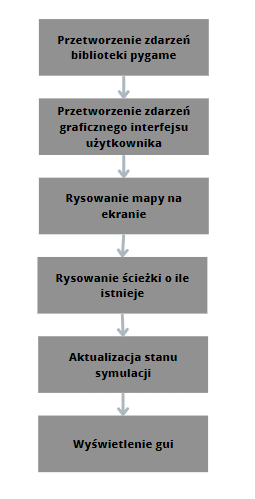
\includegraphics[width=6cm]{pages/implementacja/zdjecia/schematPetliApki.png}
	\caption{Schemat głównej pętli programu}
	\label{fig:schematPetliGlownej}
\end{figure}

Aby uprościć sobie symulowanie różnych scenariuszy i rozmiarów map otoczenia, ta ładowana jest ze wskazanego w 
programie pliku. Wskazany plik jest w formacie josn i podzielony jest na dwie sekcje. 
Pierwsza dostarcza informacje o samej mapie, natomiast druga o poruszającym się po niej robocie. Sekcja mapy zawiera lokalizacje do pliku tekstowego z zapisanymi elementami. 

\begin{lstlisting}[language=Python,caption=Uruchomienie aplikacji,label={kodPythonWczytanieMapy}]
(self.map, self.robot) = MapLoader.fromJson("maps/m02.json")
\end{lstlisting}
Ładowaniem wszystkich tych informacji zajmuje się specjalna metoda w klasie wywołana przed uruchomieniem pętli głównej. 
Wczytywana mapa jest w postaci siatki i stałym rozmiarze każdego elementu. Symulator rozróżnia kilka typów węzłów:
\begin{itemize}
	\item brak elementu - możliwy przejazd 
	\item ściana - przeszkoda do ominięcia przez algorytm
	\item punkt początkowy - punkt, od którego rozpoczyna się wyznaczanie ścieżki, zdefiniowany przez użytkownika
	\item punkt końcowy - analogicznie jak w poprzednim przypadku
	\item ścieżka - element wyznaczonej ścieżki
\end{itemize}

Wszystkie wymienione typy zapisane są w klasie Tile, reprezentującej pojedynczy rysowany i zapisywany do pliku kwadrat.
Użytkownik może w każdej chwili działania aplikacji edytować mapę. Przed zamknięciem aplikacji 
zaktualizowana mapa zapisywana jest do pliku. Wyjątkiem jest obiekt będący elementem ścieżki. 
Ten nie jest zapisywany do pliku, ponieważ generowany jest dynamicznie i służy tylko do reprezentacji wygenerowanej ścieżki.

\textbf{Wyznaczanie ścieżki i symulacja}


Po załadowaniu program oczekuje na akcje użytkownika i ewentualne uruchomienie wyznaczania ścieżki lub całej symulacji.
\begin{lstlisting}[language=Python,caption=Uruchomienie aplikacji,label={kodPythonWyznaczenieSciezki}]
elif ev.ui_element == self._startAStar:
    star = AStar(self.map.map, self.map.getSize())
    star.diagonalJump(self._diagonalJump)
    star.diagolnalCorrection(self._diagonalCorrextion)
    self.path       = star.findPath2(Node(self.map.getStartCords()), Node((self.map.getEndCords())))
    self._pathExist = True
    self.robot.stopSimulation()
    self.robot.hideRobot()
\end{lstlisting}

Po kliknięciu w przycisk odpowiadający za wyznaczenie i pokazanie ścieżki, program tworzy obiekt 
wyznaczający trasę i ustawia dodatkowe opcje algorytmu (np. skok po przekątnych). 
Dalej pobierana jest wyznaczona trasa będąca tablicą kolejnych punktów, po których należy przejść aby dojść do celu.
Na końcu ustawiana jest odpowiednia flaga programu, zatrzymywana jest symulacja i ukrywany jest robot (mamy nowo wyznaczoną trasę).
Przycisk uruchamiający symulacje sprawdza czy istnieje ścieżka i w razie potrzeby ją generuje. Następnie trasa podawana 
jest do obiektu robota odpowiadającego za symulacje i dalej symulacja jest uruchamiana.

\textbf{Przejście robota po ścieżce}

Symulator robota pobiera pierwszy punkt, do którego ma dotrzeć. Zmiana pozycji odbywa się poprzez regulator typu P z 
ustawioną nastawą na wskazany punkt. Wartość wzmocnienia proporcjonalnego wczytana jest z pliku mapy i oznaczona jest jako szybkość robota.
Dalszy etap to sprawdzenie czy symulowany robot dotarł do celu. 
\begin{lstlisting}[language=Python,caption=Uruchomienie aplikacji,label={kodPythonSprawdzenieCeluRobota}]
if abs(deltaPos0) < 0.2 and abs(deltaPos1) < 0.2:
            self._currentTarget -= 1
\end{lstlisting}
Realizowane jest to poprzez sprawdzenie czy wartość bezwzględna z różnicy aktualnej oraz docelowej pozycji jest mniejsza niż 0,1.
Po osiągnięciu punkt ustawiany jest nowy indeks wskazujący na kolejny cel.
Jeżeli na początku aktualizacji indeks jest ujemny to robot przejechał po całej wyznaczonej trasie.

\textbf{Komunikacja z robotem}
% polaczenie z robotem po tcp

Po wyznaczeniu ścieżki symulator na polecenie użytkownika może połączyć się ze zbudowanym robotem aby ten osiągnął założony cel.
Zgodnie ze schematem \cite{sch:ogolnyRozwiazania} robot po połączeniu z siecią WiFi i utworzeniu serwera TCP oczekuje na wysyłane komendy.
Aplikacja podczas uruchamiania się tworzy gniazdo, które potem zostanie wykorzystane do połączenia. 
\begin{lstlisting}[language=Python,caption=Utworzone gniazdo,label={kodPythonGniazdo}]
self._robotSocket       = socket.socket(socket.AF_INET, socket.SOCK_STREAM)
\end{lstlisting}
Dla zwiększenia elastyczności utworzone są dwa pola tekstowe pozwalające na wprowadzenie adresu ip oraz portu z uruchomionym serwerem.
Po wprowadzeniu wymaganych danych operator może spróbować nawiązać połączenie z robotem poprzez specjalny przycisk.


\begin{lstlisting}[language=Python,caption=Nawiązanie połączenia,label={kodPythonGniazdo}]
if self._robotSocketFlag is True:
self._robotSocket.close()

print(f"Laczenie z robotem {(self._textRobotIp.get_text(), int(self._textRobotPort.get_text()))}")
self._robotSocket.settimeout(1)
try:
    self._robotSocket.connect((self._textRobotIp.get_text(), int(self._textRobotPort.get_text())))
    self._robotSocketFlag = True
    self._sendCommandToRobot("setMode auto")
    print("Podlaczono!!!")
except Exception as err:
    self._robotSocketFlag = False
    print(f"Blad polaczenia z robotem")
    print(err)
\end{lstlisting}
W pierwszej kolejności sprawdzana jest flaga informująca o stanie połączenia, jeżeli jest aktywne to połączenie jest zamykane.
Na utworzonym gnieździe wywoływana jest funkcja connect z wprowadzonymi przez użytkownika parametrami.
Cała operacja zamknięta jest w bloku try..except a więc jeżeli program nie połączy się z robotem to wyświetlana jest odpowiednia informacja. 
Podczas łączenia należy zwracać uwagę na podsieci, w których jest robot i sterujący laptop. 
Dodatkowo robot posiada dynamiczne ip co zostało szerzej opisane w rozdziale o oprogramowaniu robota.
Jeżeli żaden wyjątek nie został rzucony to wysyłana jest pierwsza komenda ustawiająca tryb robota na automatyczny.


\begin{lstlisting}[language=Python,caption=Wysyłanie komendy do robota,label={kodPythonSendCmd}]
def _sendCommandToRobot(self, cmd):
    if self._robotSocketFlag is False:
        print("Robot nie podlaczony!!")
        return
    
    try:
        self._robotSocket.send(str.encode(cmd))
    except OSError as err:
        print("Robot nie podlaczony!!!")
        self._robotSocket.close()
        self._robotSocketFlag = False
        return
\end{lstlisting}
Program może wysłać dowolną komendę robota poprzez metodę sendCommandToRobot. 
Podobnie jak przy połączeniu, metoda wysyłająca dane może rzucić wyjątek o braku połączenia. W takim przypadku
wyświetlana jest odpowiednia informacja i resetowana jest flaga połączenia. 


% TODO: tu kiedys o wysyłanych komendach ze sciezka

% TODO: zdjecie z calego program, efekt
\textbf{Finalna wersja programu}

Na poniższym zrzucie widać uruchomiony program z trwającą symulacją. Po prawej stronie został umieszczony panel 
z interfejsem użytkownika. Po lewej stronie widoczna jest wczytana mapa. 
Kolorem niebieskim został oznaczony punkt startowy a czerwonym końcowy.
Żółte kratki oznaczają wyznaczoną przez algorytm ścieżkę, po której przejdzie robot. Szare pola to przeszkody, które robot ma ominąć. 
Robot oznaczony jest przez jasno-zielone koło, które przesuwa się po polu. 

\begin{figure}[H]
	\centering
	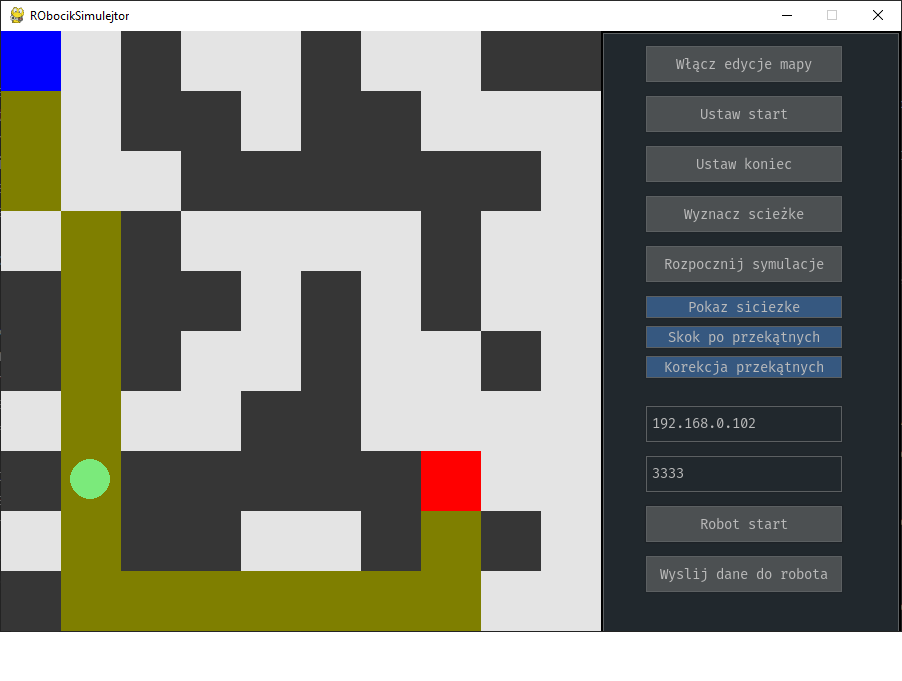
\includegraphics[width=16cm]{pages/implementacja/zdjecia/calyProgram.png}
	\caption{Widok finalnej wersji programu}
	\label{fig:finalnaWersjaProgramu}
\end{figure}

\section{Projekt robota}
\subsection{Założenia projektowe}
Wykonany robot powinien być jak najmniejszy i najprostszy w wykonaniu oraz sterowaniu tak aby móc przetestować przy jego pomocy działanie algorytmu A*. 
Robot będzie zbudowany z platformy, do której zostaną przyczepione napędy, elektronika sterująca oraz bateria. 
Do platformy zostaną przymocowane dwa gotowe moduły napędowe składające się z silnika, przekładni oraz dużego koła. 
Aby pojazd stał stabilnie, doczepione zostanie trzecie koło obracające się swobodnie w każdym kierunku.
Całość będzie sterowana przy pomocy mikroprocesora ESP32 oraz dwukanałowego sterownika silników DC opartym na układzie L298n.
Za zasilanie będzie odpowiadał litowo-jonowy akumulator 4S.

\subsection{Projektowanie zarysu robota w środowisku CAD}
Robot ma być prosty w budowie i wykonaniu, a więc założyłem, że podstawa utrzymujące pozostałe komponenty
zostanie wydrukowana na drukarce 3D. Model platformy i pozostałych posiadanych elementów został wykonany w programie Fusion 360.
Modele modułów napędowych, przedniego kółka oraz baterii pozwoliły na optymalne wyznaczenie pod względem wielkości lokalizacji wszystkich elementów.

% TODO: uprościć schematy z kicada

\begin{figure}[H]
	\centering
	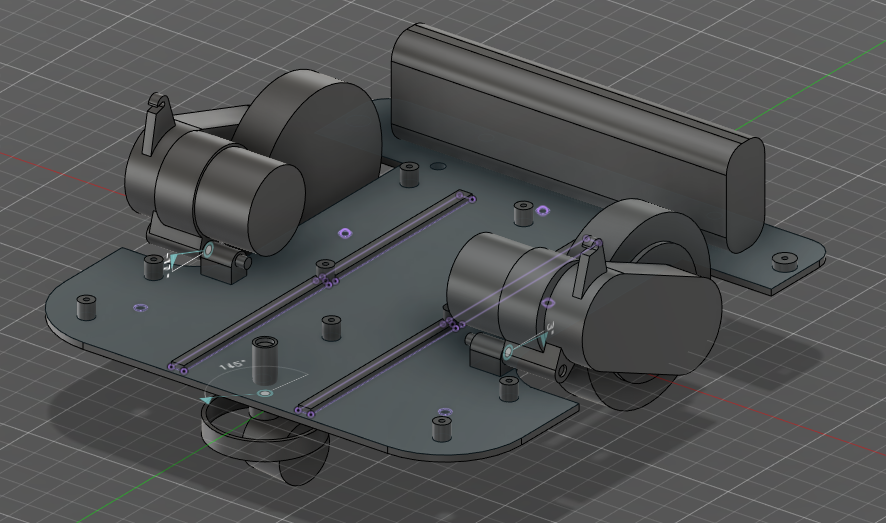
\includegraphics[width=10cm]{pages/robot/zdjecia/robotModelCaly.png}
	\caption{Zaprojektowane podwozie robota w programie Fusion360}
	\label{fig:Rys}
\end{figure}

\begin{figure}[H]
	\centering
	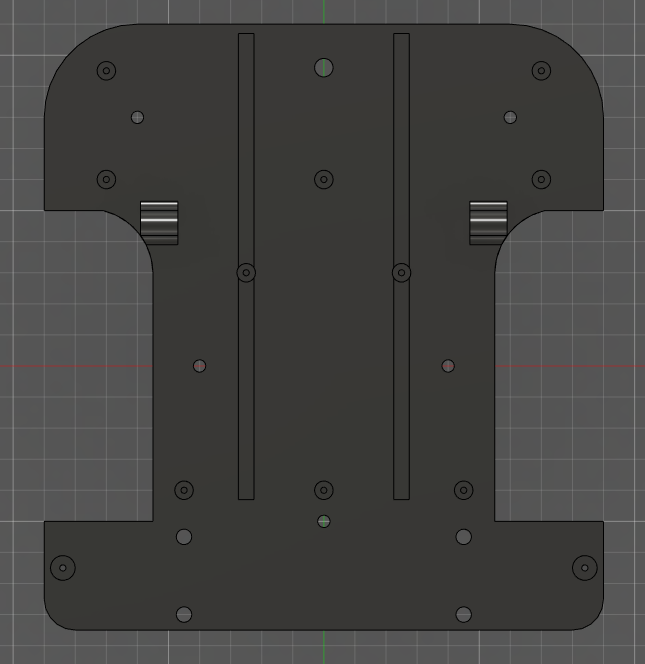
\includegraphics[width=10cm]{pages/robot/zdjecia/robotModelRama.png}
	\caption{Widok z góry na podwozie robota}
	\label{Fig:Rysunek}
\end{figure}
Model został przygotowany do druku w programie Ultimaker Cura a parametry druku zostały dobrane 
eksperymentalnie. Podstawę wydrukowano z PLA w temperaturze 220*C i wysokości warstwy 0,2mm. 
Żeby zwiększyć wytrzymałość temperatura głowicy została lekko zawyżona względem wymagań producenta filamentu.
\begin{figure}[H]
	\centering
	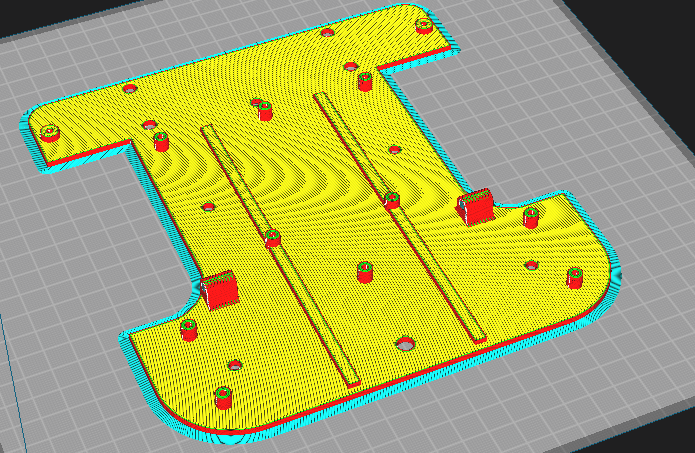
\includegraphics[width=13cm]{pages/robot/zdjecia/robotRamaCura.png}
	\caption{Widok przygotowanego do druku modelu}
	\label{fig:Rysunek}
\end{figure}
\subsection{Projekt, wykonanie oraz podłączenie elektroniki robota}
Ze względu na chęć bezprzewodowego sterowania robotem zostanie wykorzystany moduł ESP32, dla którego zostanie przygotowana odpowiednia płytka 
z wyprowadzeniami do enkoderów silnika oraz ich sterownika. Schemat elektroniczny i projekt pcb został wykonany w programie KiCad. 
\begin{figure}[H]
	\centering
	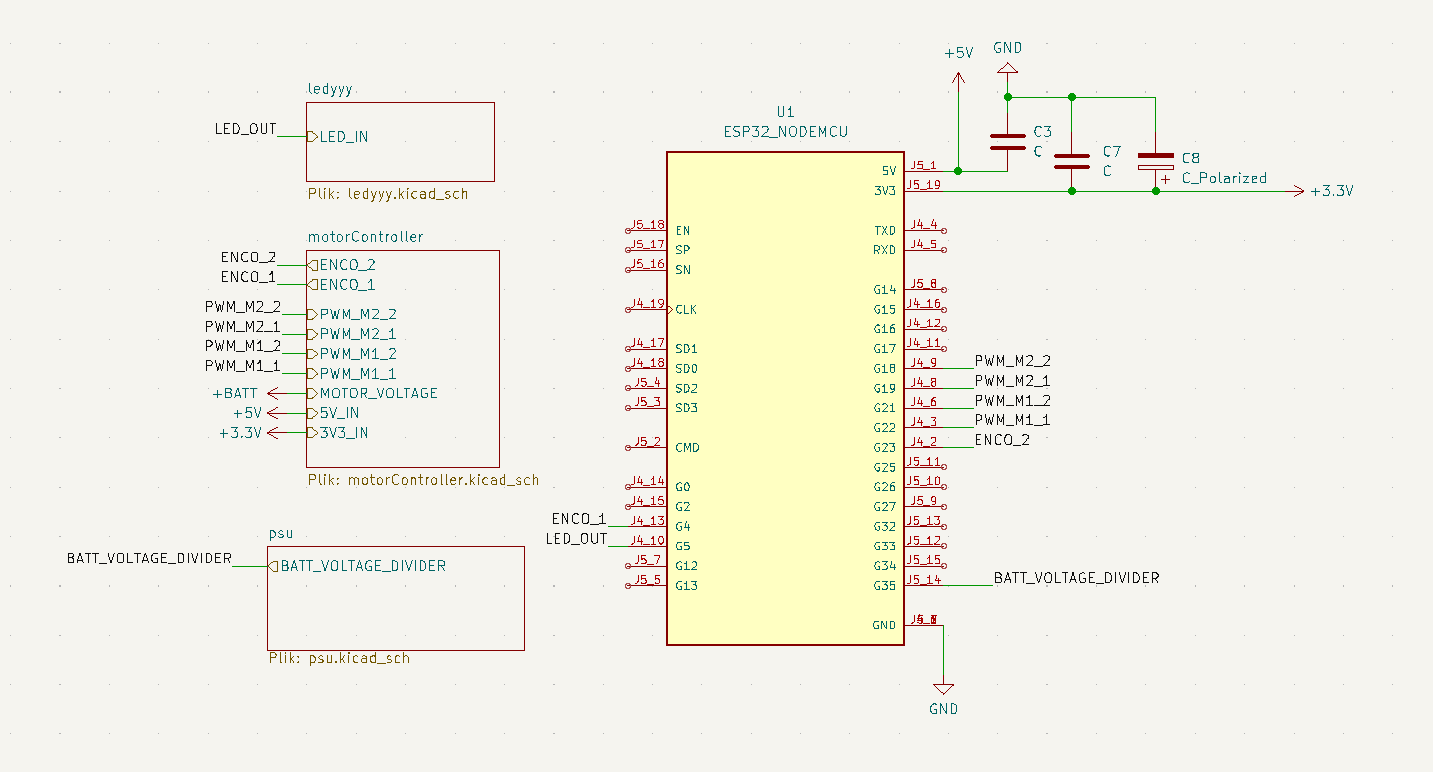
\includegraphics[width=13cm]{pages/robot/zdjecia/kicad/schematCaly.png}
	\caption{Ogólny schemat połączeń}
	\label{Fig:Rysunek}
\end{figure}
Wszystkie potrzebne elementy podsystemów mikroprocesora zostały już wlutowane w module deweloperskim,
a więc mój schemat zawiera jedynie odpowiednie połączenia z modułami roboczymi.
\begin{figure}[H]
	\centering
	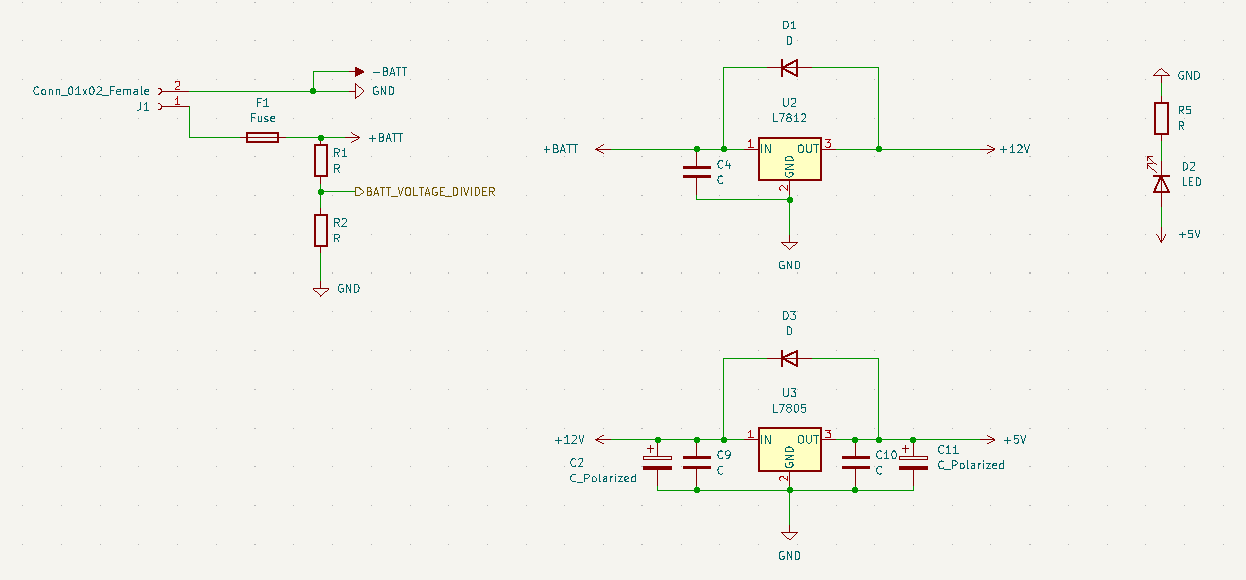
\includegraphics[width=10cm]{pages/robot/zdjecia/kicad/schematZasilanie.png}
	\caption{Ogólny schemat połączeń}
	\label{Fig:Rysunek}
\end{figure}
Użyta bateria posiada napięcie maksymalne 16,8V a więc musi zostać odpowiednio zmniejszone przed podaniem go na piny zasilania. 
Ze względu na wykorzystywaną łączność bezprzewodową a więc zwiększone zużycie prądu, zmniejszanie napięcia zostało podzielone na trzy sekcje. 
Najpierw zmniejszane jest poprzez stabilizator LM7812 z 16.8V do 12V, a następnie poprzez LM7805 z 12V napięcie redukowane jest do 5V. 
ESP32 zasilane jest napięciem 3.3V tworzonym poprzez stabilizator AMS1117 w module deweloperskim. 
Aby zredukować spadki napięć powstałe przy nagłym poborze prądu dodałem dodatkowe kondensatory filtrujące. 
Dodatkowo na schemacie widoczny jest dzielnik napięcia pozwalający na poziom naładowania baterii przez sterownik oraz programowalne diody świecące ws2812b,
jednak ostatecznie nie zostały wykorzystane w projekcie.
\begin{figure}[H]
	\centering
	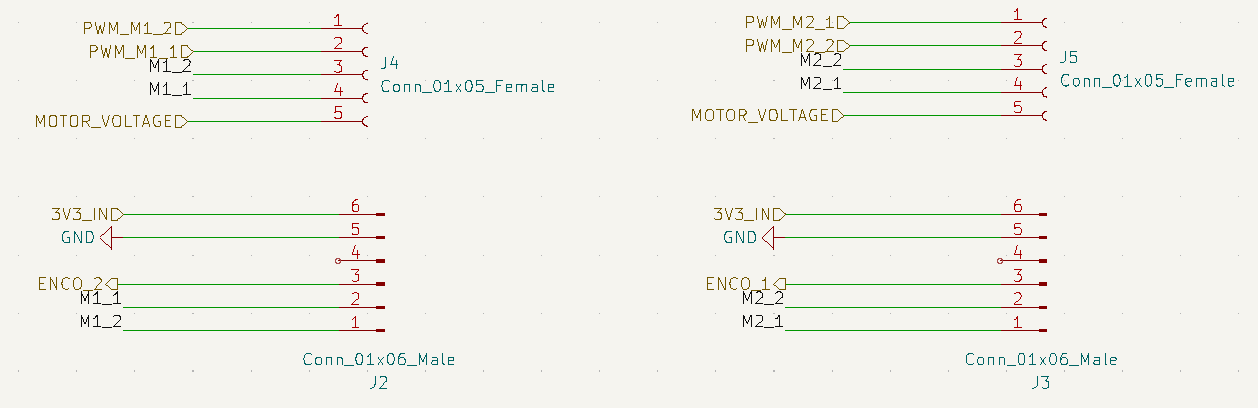
\includegraphics[width=16cm]{pages/robot/zdjecia/kicad/schematSilniki.png}
	\caption{Ogólny schemat połączeń silników}
	\label{Fig:Rysunek}
\end{figure}
Użyte moduły napędowe posiadają enkoder inkrementalny zbudowany z czujnika halla i tarczy magnetycznej zamocowanej na wale silnika.
Czujnik halla jest zasilany napięciem 3.3V i na wyjściu otrzymujemy sygnał ze "szpilkami" proporcjonalny do aktualnych obrotów silnika. 
Silniki zasilane są poprzez moduł z układem L298n, a prędkość ustalana jest poprzez odpowiednio generowany sygnał PWM. 
\begin{figure}[H]
	\centering
	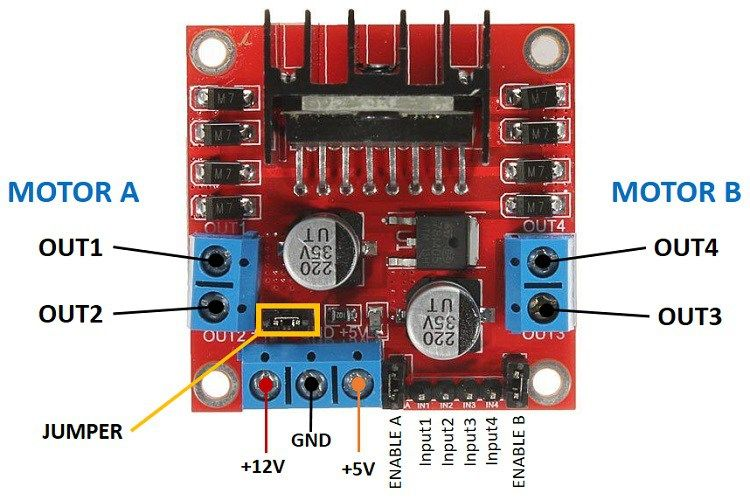
\includegraphics[width=10cm]{pages/robot/zdjecia/l298n_modul.jpg}
	\caption{Wykorzystany moduł do sterowania silnikami, L298n}
	\label{Fig:Rysunek}
\end{figure}
\begin{figure}[H]
	\centering
	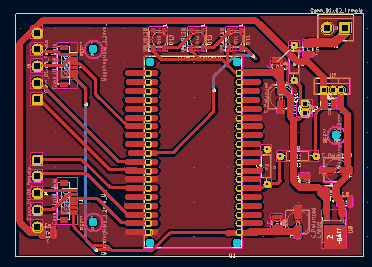
\includegraphics[width=6cm]{pages/robot/zdjecia/kicad/kiCad_PCB.png}
	\caption{Projekt PCB}
	\label{Fig:Rysunek}
\end{figure}
Na widocznym powyżej zdjęciu widać ostateczną wersje projektu pcb.


\subsection{Oprogramowanie robota}

Program sterujący robotem został napisany w C++. 
Szkielet aplikacji bazuje na projekcie utworzonym przez framework IDF w wersji 4.4 udostępnionym 
przez producenta użytego procesora. Po za tym użyta została biblioteka implementująca 
system czasu rzeczywistego FreeRTOS i ASIO do obsługi połączenia TCP. 
\begin{figure}[H]
	\centering
	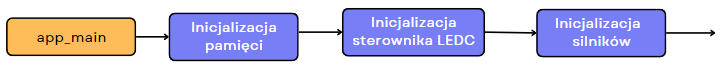
\includegraphics[width=14cm]{pages/robot/zdjecia/schematy/softSchematCz1.png}
	\caption{Schemat programu cz.1 }
	\label{Fig:Rysunek}
\end{figure}
\begin{figure}[H]
	\centering
	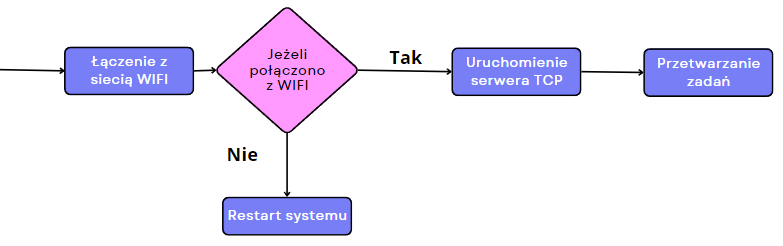
\includegraphics[width=14cm]{pages/robot/zdjecia/schematy/softSchematCz2.png}
	\caption{Schemat programu cz.2}
	\label{Fig:Rysunek}
\end{figure}

Działanie programu rozpoczyna się od wywołania funkcji app\_main, inicjalizacji funkcji systemowych i sterowników silników.
W dalszej kolejności nawiązywana jest łączność z siecią WiFi. W przypadku braku połączenia system resetuje się. 
Po poprawnym połączeniu uruchamiany jest kontekst biblioteki ASIO, a następnie uruchomienie serwera TCP.
Klienci po połączeniu do utworzonego serwera wysyłają komendy tekstowe wraz z odpowiednimi argumentami, które
robot odpowiednio przetwarza. 

\subsubsection{Sterowanie silnikami}
Sterowanie silnikami odbywa się poprzez klasę MotorController, która dziedziczy po klasie PIDController implementującej regulator PID.
Obiekt automatycznie tworzy timer uruchamiający co 100ms metodę aktualizującą wyjścia sterujące silnikiem. 
Aktualna prędkość wyznaczana jest na podstawie przerwania wyzwalanego przez enkoder silnika. Przerwanie inkrementuje licznik, 
czyszczony przez wcześniej opisany timer. Nastawy regulatora PID zostały dobrane eksperymentalnie, człon proporcjonalny wynosi 8 a całkujący i różniczkujący 0,1. 
Regulator PID możemy opisać przy pomocy wzoru:

\begin{equation}
	u(x) = e(x) * P + \int{e(x)} * I + \partial{e(x)} * D 
	\label{Eq:PID}
\end{equation}
Gdzie: $e(x)$ -- jest błędem; P,I,D -- to stałe odpowiednio członu proporcjonalnego, całkującego i różniczkującego

\begin{equation}
	e(x) = y_nast(x) - y_aktu(x)
	\label{Eq:blad}
\end{equation}
Gdzie: $y_nast(x)$ -- to nastawa regulatora, $y_aktu(x)$ -- jest rzeczywistą zmierzoną wartością
 
Powyżej przedstawiony regulator został zaimplementowany w funkcji calcOutput klasy PIDController.

\begin{lstlisting}[language=C++,caption=Zaimplementowany w C++ regulator PID,label={kodCPPPIDOutput}]
float PIDController::calcOutput(float current, float set)
{
	float error = set - current;
	float der = (error - this->_lastValue)/(_timeStep* 0.001);
	
	float output =  (this->_p * error) + 
					(this->_i * error * this->_timeStep * 0.001) + 
					(this->_d * der);

	this->_lastValue = error;
	return output;
}
\end{lstlisting}

Do wyznaczenia części różniczkującej potrzebna wartość błędu z poprzedniego wywołania pętli a ta zapisywana jest do zmiennej prywatnej klasy lastValue. 
Całkowanie zrealizowane jest poprzez pomnożenie przez krok dyskretyzacji. Stałe regulatora ustawiane są poprzez wywołanie konstruktora klasy.

Tak zaimplementowany regulator używany jest do wyznaczenia sygnału PWM, bezpośredniego sterującego układem L298n a ten silnikami. 

\begin{lstlisting}[language=C++,caption=Wyznaczenie modulacji PWM,label={kodCPPPWM}]
if(abs(setSpeed) - 1 > 0) // jezeli predkosc jest wieksza to pid jak nie to hamulec bo pwm=0
{
	pidToPwm = (int) this->calcOutput(abs(this->getCalculatedEngineRadialSpeed()), abs(setSpeed));
	if(setSpeed < 0)
	{
		pwmCh = 1;
	}
	else
		pwmCh = 0;

	pidToPwm += ledc_get_duty(LEDC_LOW_SPEED_MODE, this->_chanels[pwmCh]);
	pidToPwm = std::min(pidToPwm, 8192);
	pidToPwm = std::max(pidToPwm, 0);
}

// ustawienie wyjsc
ledc_set_duty(LEDC_LOW_SPEED_MODE, this->_chanels[pwmCh], (int)pidToPwm);
ledc_update_duty(LEDC_LOW_SPEED_MODE, this->_chanels[pwmCh]);

// ustawienie drugiego kanalu
ledc_set_duty(LEDC_LOW_SPEED_MODE, this->_chanels[(pwmCh==0)?1:0], 0);
ledc_update_duty(LEDC_LOW_SPEED_MODE, this->_chanels[(pwmCh==0)?1:0]);
\end{lstlisting}

W pierwszej kolejności sprawdzana jest zadana prędkość, jeżeli ta jest zbyt niska to na piny wystawiane są bezpośrednio stany niskie.
Jeżeli ustawiona prędkość jest poprawna to wyznaczamy wyjście regulatora. Sterowanie kierunkiem obrotów odbywa 
się poprzez znak zadanej prędkości a więc regulator otrzymuje wartości bezwzględne. 
Wyjście regulatora PID sumowane jest z aktualną nastawą. Wyjścia pwm skonfigurowane są w częstotliwości 5kHz i rozdzielczości 13bitów. 
Przed wysłanie nastaw do kontrolera pwm, te są obcinane do obsługiwanych zakresów (tj. 0 - 8192).

\subsubsection{Serwer TCP}

Po podłączeniu zasilania i uruchomieniu systemu robot oczekuje na polecenia wysłane do robota poprzez protokół internetowy TCP. Serwer został napisany w oparciu o bibliotekę ASIO, pozwalającą na asynchroniczną obsługę wejścia i wyjścia (w tym sieci).
\begin{figure}[H]
	\centering
	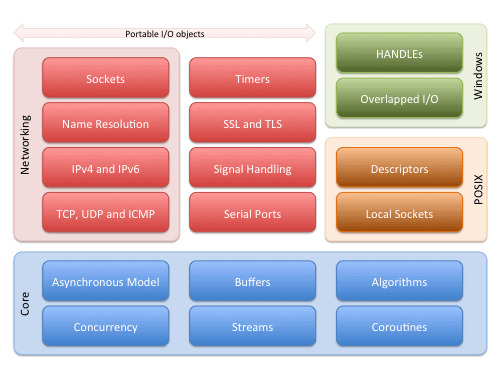
\includegraphics[width=10cm]{pages/robot/zdjecia/schematASIO.jpg}
	\caption{Schemat biblioteki ASIO \cite{asio}}
	\label{Fig:schematASIO}
\end{figure}
Biblioteka została napisana w C++ i pracuje w oparciu o standard POSIX wspierany również przez wykorzystywane ESP32.
Do akceptacji przychodzących połączeń została napisana klasa Server. Konstruktor przyjmuję referencje do kontekstu utworzonego w funkcji głównej programu. 
Uruchomienie kontekstu jest ważną częścią biblioteki ASIO, przetwarzane są w niej wszystkie asynchroniczne operacje.
Aby zapewnić jak najlepszy czas przetwarzania, kontekst uruchomiony jest w oddzielnym wątku przyłączonym do drugiego fizycznego rdzenia.

\begin{figure}[H]
	\centering
	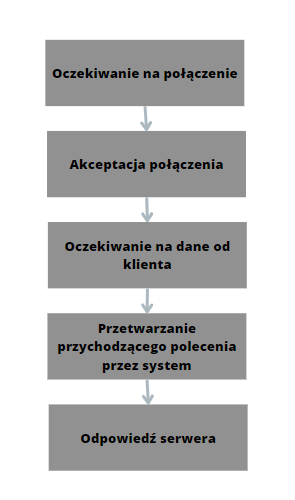
\includegraphics[width=6cm]{pages/robot/zdjecia/schematTCP.png}
	\caption{Schemat działania serwera TCP}
	\label{Fig:schematSerweraTCP}
\end{figure}

Po zaakceptowaniu przychodzącego połączenia, obiekt połączenia dodawany jest do specjalnej tablicy przechowującej wszystkich klientów. 
Dane mogą być równocześnie przetwarzane w kilku miejscach a więc używane są dzielone wskaźniki, które automatycznie usuwają dane jeżeli nikt z nich nie korzysta.
Na każdym aktywnym połączeniu prowadzony jest nasłuch, dzięki czemu możemy mieć równocześnie podłączony program do generowania ścieżki i drugi pozwalający na podgląd parametrów robota.
Klient wysyła polecenia w formie tekstowej, te przekazywane są do klasy systemowej odpowiednio interpretujące ich przeznaczenie.
Jeżeli komenda tego wymaga (np. zwrócenie prędkości obrotowej silników) to dane są odsyłane do klienta w postaci tekstu i oddzielonych przerwą liczb. 

% TODO: nawiązanie do serwera dhcp
	
\section{Przeprowadzone testy}


\subsection{Test poprawności trasowania}

\subsection{Wpływ ustawień na wyznaczoną ścieżkę}

\subsection{Sprawdzenie wpływu funkcji heurestycznej na ścieżkę}

\subsection{Test komunikacji z fizycznym robotem}



\clearpage
	
\addcontentsline{toc}{section}{Literatura}
	
\begin{thebibliography}{4}
	\bibitem{dokESP32} https://docs.espressif.com/projects/esp-idf/en/latest/esp32/get-started/index.html. Dostęp 04.01.2023.
	\bibitem{robotShakey} https://medium.com/dish/75-years-of-innovation-shakey-the-robot-385af2311ec8 Dostęp 04.01.2023.
	\bibitem{dokPygame} https://www.pygame.org/docs/ Dostęp 06.01.2023
	\bibitem{dokPygameGui} https://pygame-gui.readthedocs.io/en/latest/ Dostęp 06.01.2023
	\bibitem{asio} https://think-async.com/Asio/ Dostęp 06.01.2023
	\bibitem{RRTLec} https://www.cs.cmu.edu/~motionplanning/lecture/lec20.pdf Dostęp 10.01.2023
	\bibitem{SLAMMat} https://www.mathworks.com/discovery/slam.html Dostęp 10.01.2023
\end{thebibliography}
	
\clearpage
	
% \makesummary
\end{document} 